\subsection{OB-2 (ADU)}
Správa disků a souborových systémů (zařízení, souborové systémy UFS (EXT) a ZFS, disková pole RAID, diskové kvóty), síťové souborové systémy (NFS, CIFS), swap v unixových operačních systémech.

\textbf{Zařízení:}
\begin{itemize}
    \item popsána speciálními soubory v adresáři /dev
    \item znakové/blokové
    \item zápis/čtení souboru znamená stejnou operaci nad zařízením
    \item pseudozařízení --- /dev/null, /dev/random, /dev/zero,...
    \item vše potřebné uloženo v i-node (jako odkaz na driver)
    \item většinou může operace nad těmito soubory provádět jen root
    \item lze vytvořit přes mknod
\end{itemize}

\textbf{Disky:}
\begin{itemize}
    \item rozdělení disku závisí na HW i na OS
    \item na x86: partitions (partition tabulka)
    \item na solaris: slices (pokud na x86, jsou v rámci partitions)
    \item Partitions:
    \begin{itemize}
        \item rozdějují fyzický disk na více logických celků
        \item popsány partition tabulkou
        \item MBR --- Master Boot Record --- v prvním sektoru disku, obsahuje kód zavaděče (GRUB) a partition tabulku se 4 záznamy (max 4 partitions)
        \item GPT --- GUID Partition Table --- partitions mají globálně unikátní ID, je součástí UEFI (nástupce BIOS)
    \end{itemize}
\end{itemize}

\textbf{Filesystem:}
\begin{itemize}
    \item logický --- adresářový strom
    \item fyzický --- filesystém na disku, připojuje se k mountovacímu bodu
    \item diskový, síťový, ...
\end{itemize}

\textbf{SWAP:}
\begin{itemize}
    \item odkládací prostor na disku pro nepoužívané stránky paměti
    \item většinou se řeší buď pomocí swap partition, nebo swapovacími soubory
\end{itemize}

\textbf{UFS}
\begin{itemize}
    \item efektivní pro menší soubory (max desítky/stovky MB)
    \item nevzniká fragmentace
    \item bootblock (na začátku disku), superblock primární (po bootblocku) a záložní (na začátku každé cylindr grupy)
    \item i-node
    \begin{itemize}
        \item struktura obsahující metadata
        \item typ, přístupová práva, vlastník, skupina, velikost, čas vytvoření, přístupu a modifikace, čítač linků
        \item odkazy na datové bloky: 12 přímých, 3 nepřímé (první, druhé a třetí úrovně)
    \end{itemize}
    \item příkazy: mkfs (vytvoření filesystému), mount (připojení FS k mountovacímu bodu), fsck (kontrola a oprava disku)
    \item snapshot --- zapamatování stavu FS, používá se k archivaci
\end{itemize}

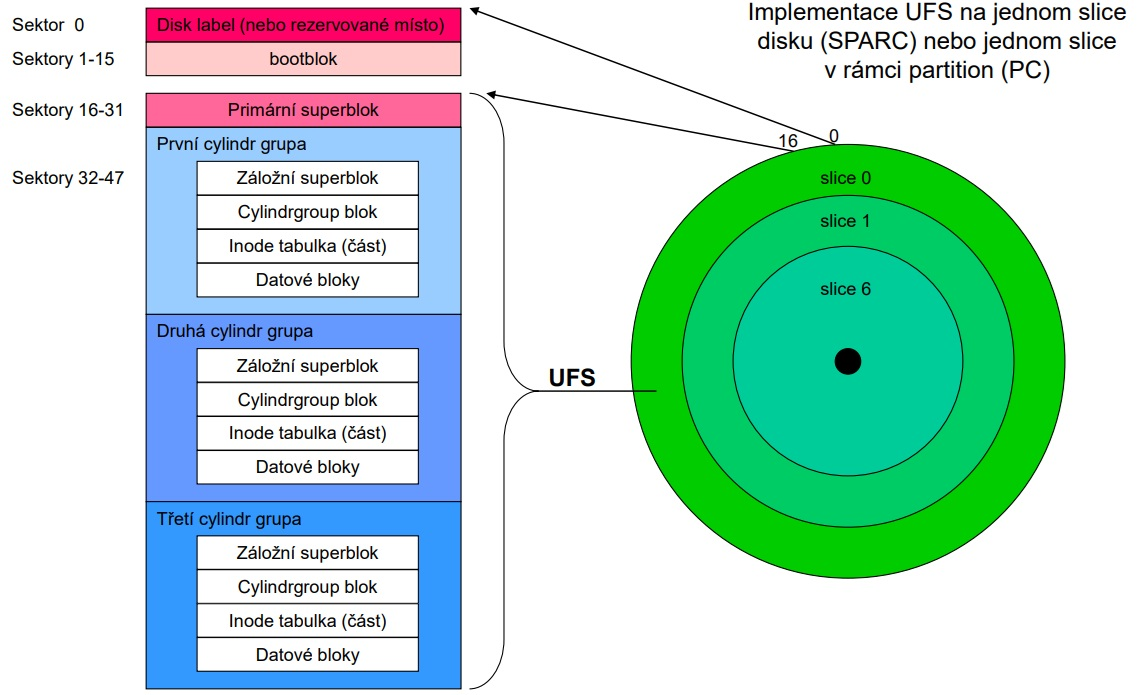
\includegraphics[width=0.8\textwidth]{img/OB-2_0.jpg}

\textbf{RAID}
\begin{itemize}
    \item Redundant Array of Independent Disks
    \item možné řešit jak HW tak SW
    \item složení jednoho logického disku z více fyzických
    \item může zvýšit kapacitu, zvýšit výkon a zvýšit bezpečnost (obrana proti výpadku)
    \item RAID 0 - zřetězení (JBOD - just a bunch of disks)
    \begin{itemize}
        \item data se ukládají postupně na disky za sebe --- když se zaplní jeden, začne se ukládat na druhý
        \item redundance 0 \%
        \item výpadek jednoho disku způsobí ztrátu dat
        \item výkon se nemění
    \end{itemize}
    \item RAID 0 - prokládání
    \begin{itemize}
        \item data jsou ukládána cyklicky po blocích na jednotlivé fyzické disky
        \item redundance 0 \%
        \item výpadek jednoho disku způsobí ztrátu všech dat
        \item výkon zvýší $m$ krát ($m$ je počet disků)
    \end{itemize}
    \item RAID 1 - zrcadlení
    \begin{itemize}
        \item stejná data jsou uložena na všech discích
        \item redundance je $100\times (m-1)/m$ \%
        \item data přežijí výpadek $m-1$ disků a výkon nebude degradován
        \item write operace stejně rychlé, read se může zrychlit až $m$ krát
    \end{itemize}
    \item RAID 1+0 / 0+1
    \begin{itemize}
        \item nejvyšší logický disk je rozdělen podle RAID 0/1, nižší logické disky jsou opačně (RAID 1/0)
        \item redundance je podle počtu zrcadlení v RAID 1 části --- při 2 kopiích dat je to 50 \%
        \item data přežijí výpadek od 1 do $m/2$ disků (př 2 kopiích)
        \item write operace zrychleny až $m/2$ krát, read až $m$ krát
    \end{itemize}
    \item RAID 2, 3, 4 se nepoužívají (2: prokládání po bitech + hammingův kód, 3: prokládání po bytech a zabezpečení pomocí uložení parity uložené na jednom fyzickém disku, 4: prokládání po blocích, uládání parity na jednom fyzickém disku)
    \item RAID 5
    \begin{itemize}
        \item prokládání po blocích na $m$ fyzických discích + ukládání parity cyklicky ukládané na jednotlivých discích
        \item redundance je $100/m$ %
        \item data přežijí výpadek jednoho disku, ale bude degradován výkon
        \item read se zrychlí, write pomalejší
    \end{itemize}
    \item RAID 6
    \begin{itemize}
        \item prokládání po blocích na $m$ fyzických discích + ukládání dvojí parity cyklicky ukládané na jednotlivých discích
        \item redundance je $200/m$ %
        \item data přežijí výpadek dvou disků, ale bude degradován výkon
        \item read se zrychlí, write pomalejší
    \end{itemize}
\end{itemize}

\textbf{ZFS}
\begin{itemize}
    \item snaží se řešit problémy stávajících FS
    \begin{itemize}
        \item nekonzistence při nekorektním vypnutí
        \item nemožnost/komplikované zvětšování kapacity FS
        \item RAID, snapshot, zálohování jsou řešené mimo vlastní FS
        \item FS nejsou hierarchické
        \item komplikovaná administrace
        \item chybějící klonování, cache, kryptování, deduplikace...
    \end{itemize}
    \item metadata řešena podobně jako v UFS
    \item datový prostor tvoří virtuální datová oblast --- pool
    \item pool je tvořen zdroji dat --- disky, partitions, soubory (speciální --- zařízení)
    \item z poolu se alokují datové bloky --- různá velikost, tvořené nad strukturami RAID
    \item transakční systém "copy on write" --- data se nepřepisují, pouze se zkopírují, změní a pak je změna přijata či zamítnuta
    \item pool sám je (ZFS) FS
    \item každý blok má kontrolní součet
\end{itemize}

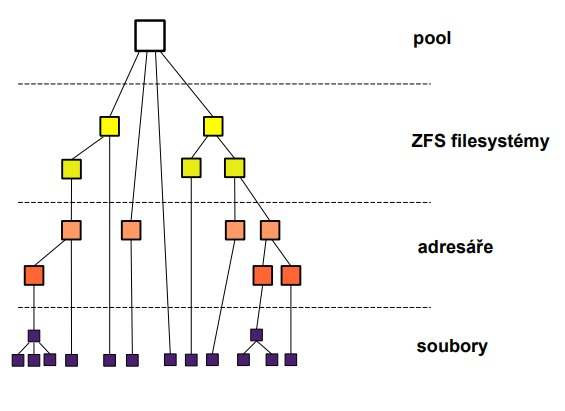
\includegraphics[width=0.8\textwidth]{img/OB-2_1.jpg}

\textbf{NFS}
\begin{itemize}
    \item daemons na serveru:
    \begin{itemize}
        \item mountd --- vyřizuje požadavky na mount, vrací file handle
        \item nfsd --- vyřizuje požadavky na operace se soubory, vrací data
        \item statd --- spolupracuje s lockd, znovunastavuje spojení po výpadku
        \item lockd --- zamykání NFS souborů, požadavek se posílá z klienta na server
        \item nfslogd --- logování přístupů
    \end{itemize}
    \item daemons na klientu --- statd, lockd
    \item NFS 2/3 nestavové, NFS 4 stavový
    \item NFS 4 --- sjednocený daemon, well known port 2049, delegace cache, možnost mountovat pseudo filesystém (vyšší adresář, ale s přístupem jen do nižšího)
\end{itemize}

\textbf{CIFS/SMB} (Samba) je novější síťový FS, snadnější vazba unix-windows.